\chapter{Progettazione}
\label{ch:progg}

Il lavoro di progettazione è diviso in due parti strettamente collegate: prima la definizione delle API, che vengono esposta al client, dopo la progettazione del database. Durante le fasi di implementazione e test è spesso capitato di raffinare dettagli riguardo sia le API che il database, tuttavia il grosso del lavoro è stato svolto prima dell'implementazione.

\section{API}

Gli utenti possono interagire con SeismoCloud utilizzando l'applicazione mobile o l'applicazione Web. Tali applicazioni comunicano con il server utilizzando il protocollo HTTPS, seguendo lo stile architetturale REST. Affinché sia comprensibile le ragioni dietro la progettazione delle API, viene descritta brevemente l'architettura REST e lo strumento di progettazione vero e proprio, cioè la specifica OpenAPI.

\paragraph{Architettura REST} La \textit{representational state transfer} (REST) \cite{rest} è uno stile architetturale basato su HTTP \cite{http}. Un sistema di definisce \textit{RESTful} se implementa lo stile architetturale REST. Pur non essendo uno standard, un sistema \textit{RESTful} utilizza degli standard, nel caso di SeismoCloud: HTTP per la comunicazione, URI \cite{uri} per l'identificazione della risorsa e JSON \cite{json} per la rappresentazione della risorsa.

Affinché un sistema sia definibile \textit{RESTful}, è necessario che rispetti sei vincoli, di cui uno opzionale. Di seguito viene dato l'elenco e viene indicato come e se SeismoCloud soddisfa i vincoli, considerando sia le API già esistenti sia quelle progettate per l'occasione:

\begin{itemize}
\item \textbf{Client-server}: il client e il server devono essere dei sistemi indipendenti, uniti tramite delle interfacce. Poiché SeismoCloud effettua questa divisione tra client e server, soddisfa il vincolo.
\item \textbf{Stateless}: la comunicazione tra client e server non prevede il concetto di sessione. HTTPS è un protocollo di sua natura senza concetto di sessione, per cui tutte le informazioni necessarie al client o al server per soddisfare una richiesta sono contenute all'interno della singola comunicazione. SeismoCloud, e quindi le API, soddisfa questo vincolo.
\item \textbf{Cacheable}: le risposte del server devono essere costruite in modo da facilitare il loro riutilizzo, attraverso l'uso della cache (a livello del client o del server). SeismoCloud soddisfa questo vincolo, anche se alcune risposte delle API, in particolare quelle che dipendono dal tempo o dal singolo utente, non sono pensate per essere riutilizzate.
\item \textbf{Layered system}: il client non può sapere se è connesso direttamente al server che eroga le API o a un sistema intermedio. Nell'architettura di SeismoCloud, pur se non mostrato nella figura \ref{fig:architettura}, sono presenti dei server intermedi prima che una richiesta raggiungano gli applicativi che erogano effettivamente le API, per cui soddisfa il vincolo.
\item \textbf{Uniform interface}: letteralmente indica che le interfacce devono essere uniformi. Può significare molte cose, tra cui l'indipendenza tra il come vengono salvati i dati in un database e come vengono erogati al client, oppure la condizione per cui ogni API sia processabile in modo indipendente. SeismoCloud, come si vedrà anche in seguito, soddisfa questo vincolo.
\item \textbf{Code on demand}: l'unico vincolo \textbf{opzionale}, prevede di estendere o personalizzare le funzionalità di un client trasferendo codice eseguibile. SeismoCloud non soddisfa questo vincolo.
\end{itemize}

REST si basa sull'esistenza di risorse, che possono essere documenti o file identificati da un URL. Il client può accedere alla risorsa fornendo l'URL che la identifica e un'operazione da applicare, che corrispondono ai metodi HTTP (i più comuni sono \texttt{GET}, \texttt{POST}, \texttt{PUT}, \texttt{DELETE}). Nella realtà il client accede a una rappresentazione della risorsa, che può avvenire in varie forme in base al \textit{media type}, una stringa che identifica il formato che rappresenta la risorsa (a esempio JSON o XML). Solitamente le risorse sono organizzate in collezioni e il client può agire su quest'ultimo oltre che sulle risorse.

La tabella \ref{tab:rest} mostra la relazione tra i metodi HTTP e URL \cite{http-methods}. SeismoCloud segue questa relazione, l'unica differenza importante è che le API utilizzano il metodo \texttt{PUT} al posto di \texttt{POST} quando si agisce sulle collezioni. Questa caratteristica del sistema è stata seguita anche nelle API progettate, pur mantenere una consistenza interna anche se concettualmente errata.

\texttt{https://api.example.com/chats/} è un esempio di URL che identifica una collezione, \texttt{https://api.example.com/chats/3423} identifica una specifica risorsa all'interno della collezione.

\begin{table}[h!]
\centering
\caption{Semantica dei metodi HTTP e URL.}
\label{tab:rest}

\begin{tabular}{c|p{14em}|p{14em}}
\textbf{Metodo} & \textbf{URL collezione} & \textbf{URL risorsa} \\
\hline
GET & Restituisce l'elenco delle risorse. & Restituisce la risorsa. \\
PUT & Sostituisce l'intera collezione. & Sostituisce o crea la risorsa. \\
POST & Crea una risorsa nella collezione. & Vedi PUT. \\
DELETE & Elimina l'intera collezione. & Elimina la risorsa. \\
\end{tabular}
\end{table}

\paragraph{OpenAPI} Il frammento di codice \ref{listing:openapi} mostra come viene definita nella specifica OpenAPI 3.0 \cite{openapi}, conosciuta in origine come specifica Swagger, l'API \texttt{GET /seismometers/}. Tale specifica permette di progettare API RESTful in modo \textit{machine-readable format}, cioè che siano processabili dal computer. I software che implementano la specificano possono essere utilizzati per diversi scopi, tra cui la generazione automatica di codice implementativo o di test, il controllo semantico delle API, la generazione della documentazione in vari formati e molto altro. In SeismoCloud OpenAPI viene utilizzato per fini documentativi. Il vantaggio principale è che le API possono essere progettate e documentate in un semplice file testuale, modificabile da qualsiasi editor di testo e convertibile in altri formati. La figura \ref{fig:openapi-render} mostra la conversione automatica dalla specifica a codice HTML per la documentazione.

In SeismoCloud il file della specifica è realizzato in formato standard YAML \cite{yaml} e utilizza versione 3.0 della specifica. Per ogni URL vengono elencate le operazioni (\texttt{GET}, \texttt{POST}...) e per ognuna si specificano gli eventuali parametri nel percorso o nella query, l'eventuale body e le possibili risposte. Quando si coinvolgono degli schemi, come mostrato nel frammento in \texttt{callback}, OpenAPI utilizza un sottoinsieme arricchito della specifica JSON Schema \cite{json-schema}, per indicare il tipo, la lunghezza o altre caratteristiche del dato.

\afterpage{\clearpage} % Aiuta il posizionamento dei float.

\begin{figure}[ht]
\centering
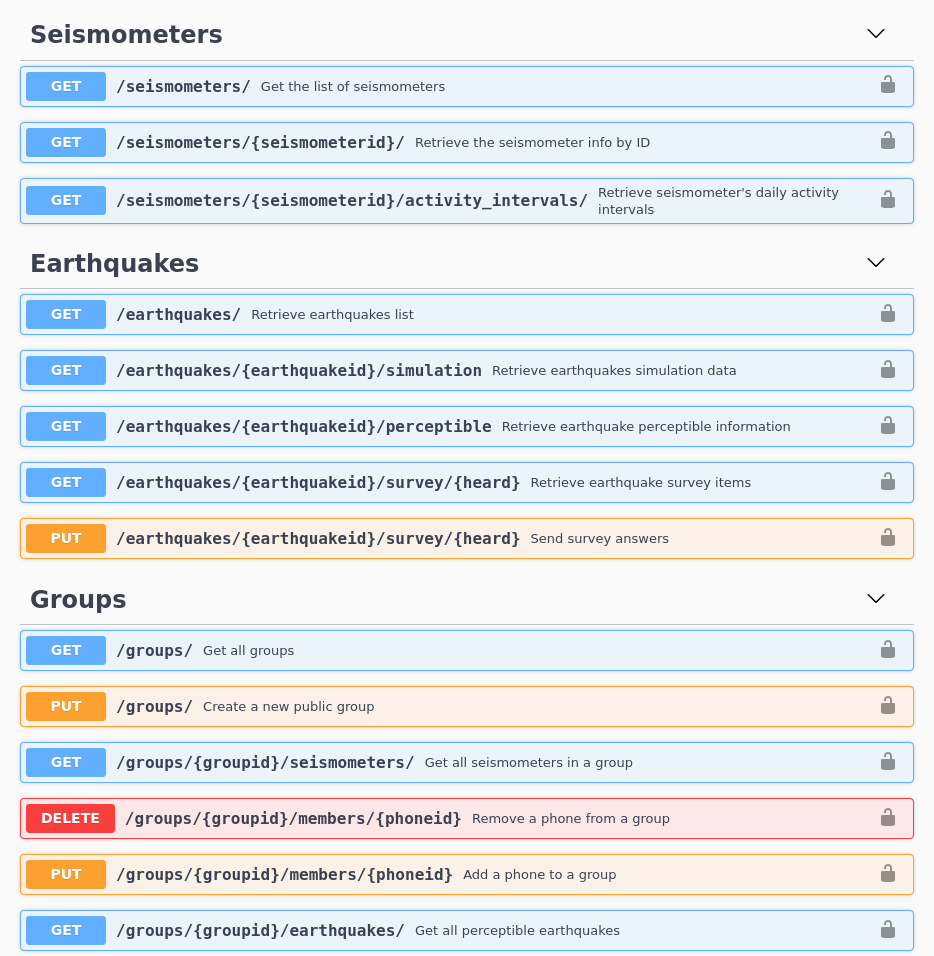
\includegraphics[width=\textwidth]{assets/03/openapi.png}
\caption{Conversione del file testuale delle API in HTML.}
\label{fig:openapi-render}
\end{figure}

\begin{longlisting}
\begin{minted}{yaml}
paths:
  # Seismometers
  /seismometers/:
    parameters:
      - $ref: "#/components/parameters/XPhoneID"
      - $ref: "#/components/parameters/XAppBuild"
      - $ref: "#/components/parameters/XAppVersion"
      - $ref: "#/components/parameters/XAppLanguage"
      - $ref: "#/components/parameters/XAppPlatform"
    get:
      tags: ["Seismometers"]
      operationId: getSeismometers
      summary: Get the list of seismometers
      description: |-
        The response contains the list of all seismometers. If the user is not
        the owner of the sensor, the position might be scrambled due to privacy
        flag.
      security:
        - OpenID: []
      parameters:
        - name: callback
          in: query
          schema: { type: string }
          required: false
          description: Callback JSONP function name
      responses:
        '200':
          description: Seismometer list available
          content:
            application/json:
              schema:
                type: array
                items:
                  $ref: '#/components/schemas/Seismometer'
        '400': { $ref: '#/components/responses/BadRequest' }
        '500': { $ref: '#/components/responses/InternalServerError' }
\end{minted}
\caption{Specifica di \texttt{GET /seismometers/} in OpenAPI 3.0.}
\label{listing:openapi}
\end{longlisting}

\paragraph{API} Per implementare la funzionalità di messaggistica sono state progettate 9 API REST, riassunte nella tabella \ref{tab:api}. Le risorse esposte al client sono le chat, il nome utente, i messaggi e le sottoscrizioni. Su tali risorse e relative collezioni il client non può operare con tutti i metodi, ma solo con quelli permessi.

Sono state seguite strettamente le convenzioni utilizzate nelle altre API di SeismoCloud, ciò ha influito la scelta dei codici di stato restituiti, la formazione dei percorsi, l'uso del metodo \texttt{PUT} al posto di \texttt{POST} nella creazione di risorse all'interno di una collezione (per esempio in \texttt{PUT /chats/\{chatid\}/messages/}).

\begin{table}[ht!]
\centering
\caption{Elenco riassuntivo delle API progettate.}
\label{tab:api}

\begin{tabular}{c|c|p{16em}}
\textbf{Metodo} & \textbf{URL} & \textbf{Descrizione} \\
\hline
GET & /chats/ & Restituisce un elenco delle ultime chat aggiornate. \\
PUT & /chats/ & Crea una nuova chat. \\
GET & /chats/\{chatid\}/messages/ & Restituisce un elenco dei messaggi della chat. \\
PUT & /chats/\{chatid\}/messages/ & Crea un messaggio in una chat. \\
GET & /images/\{imageid\} & Recupera l'immagine. \\
GET & /me/username & Recupera il nome utente. \\
PUT & /me/username & Imposta il nome utente. \\
DELETE & /me/chats/subscribed/\{chatid\} & Elimina la sottoscrizione a una chat. \\
PUT & /me/chats/subscribed/\{chatid\} & Crea la sottoscrizione a una chat.
\end{tabular}
\end{table}

\paragraph{Schemi} In aggiunta alle API sono stati definiti gli schemi che possono essere restituiti o che il client deve inserire nella chiamata affinché vada a buon fine. Gli schemi consistono in tipi primitivi, come interi e stringe, o composti, come oggetti e liste. Affinché il client utilizzi in modo corretto le API è importante definire e documentare tali schemi. La tabella \ref{tab:schemi} riassume tutti gli schemi utilizzati nelle API sopracitate.

I tipi primitivi \texttt{EarthquakeID}, \texttt{Latitude} e \texttt{Longitude} sono già preesistenti nel progetto, mentre gli altri sono stati definiti per l'occasione. I tipi primitivi, come \texttt{SliderValue} o \texttt{TextValue}, sono specializzazioni dei tipi come interi o stringhe.

Gli unici tipi composti disponibili sono gli oggetti \texttt{Message} e \texttt{Chat}, con gli attributi mostrati nella tabella \ref{tab:chat_message}. In \texttt{Message}, Il client può distinguere il tipo del messaggio controllando l'attributo \texttt{type} per poi accedere all'attributo corrispondente al tipo. In caso di un'immagine viene indicato il suo identificativo per ottenere l'immagine con \texttt{GET /images/\{imageid\}}. In \texttt{Chat}, l'attributo \texttt{latestMessage} è opzionale perché una chat appena creata potrebbe non contenere alcun messaggio; la funzione di tale attributo è permettere l'anteprima del messaggio nell'elenco delle chat. L'attributo \texttt{eartquakeID} è opzionale perché una chat potrebbe non avere associato alcun terremoto. Non è possibile inviare un messaggio in una chat chiusa. Le coordinate indicano la zona approssimativa in cui la chat è stata creata.

\begin{table}[ht!]
\centering
\caption{Elenco riassuntivo schemi utilizzati dalle API.}
\label{tab:schemi}

\begin{tabular}{c|c|c|p{14em}}
\textbf{Nome} & \textbf{Tipo} & \textbf{Formato} & \textbf{Descrizione} \\
\hline
ChatID & \texttt{integer} & \texttt{int64} & Identificativo di una chat. \\
MessageID & \texttt{integer} & \texttt{int64} & Identificativo di un messaggio. \\
ImageID & \texttt{string} & \texttt{UUID} & Identificativo di un'immagine. \\
EarthquakeID & \texttt{integer} & \texttt{int64} & Identificativo interno di un terremoto. \\
Latitude & \texttt{number} & --- & Latitudine in gradi. \\
Longitude & \texttt{number} & --- & Longitudine in gradi. \\
Username & \texttt{string} & --- & Nome utente mostrato nei messaggi. \\
SliderValue & \texttt{integer} & --- & Valore dello slider. \\
TextValue & \texttt{string} & --- & Contenuto di un messaggio testuale. \\
Image & \texttt{string} & \texttt{binary} & L'immagine in formato binario. \\
Message & \texttt{object} & --- & Singolo messaggio in una chat. \\
Chat & \texttt{object} & --- & Singola chat.
\end{tabular}
\end{table}

\afterpage{\clearpage}

\begin{table}[ht!]
\centering
\caption{Attributi degli schemi \texttt{Chat} e \texttt{Message}.}
\label{tab:chat_message}

\begin{tabular}{c|c|c|p{17em}}
\hline
\multicolumn{4}{c}{\textbf{\texttt{Message}}} \\
\hline
\textbf{Nome} & \textbf{Tipo} & \textbf{Formato} & \textbf{Descrizione} \\
\hline
id & \texttt{MessageID} & --- & Obbligatorio, identificativo di un messaggio. \\
createdAt & \texttt{string} & \texttt{date-time} & Obbligatorio, data e ora di invio del messaggio. \\
sentBy & \texttt{Username} & --- & Obbligatorio, nome utente di chi ha inviato il messaggio. \\
type & \texttt{string} & \texttt{enum} & Obbligatorio, con valori possibili \texttt{text}, \texttt{image} o \texttt{slider}, indica il tipo del messaggio inviato. \\
text & \texttt{TextValue} & --- & Contenuto testuale, che può essere un messaggio di testo o l'identificativo di un'immagine. \\
slider & \texttt{SliderValue} & --- & Valore dello slider.
\end{tabular}

\bigskip

\begin{tabular}{c|c|c|p{17em}}
\hline
\multicolumn{4}{c}{\textbf{\texttt{Chat}}} \\
\hline
\textbf{Nome} & \textbf{Tipo} & \textbf{Formato} & \textbf{Descrizione} \\
\hline
id & \texttt{ChatID} & --- & Obbligatorio, identificativo di una chat. \\
name & \texttt{string} & --- & Obbligatorio, nome della chat. \\
createdAt & \texttt{string} & \texttt{date-time} & Obbligatorio, data e ora di creazione della chat. \\
closed & \texttt{boolean} & --- & Obbligatorio, indica se la chat è stata chiusa. \\
subscribed & \texttt{boolean} & --- & Obbligatorio, indica se l'utente è sottoscritto alla chat. \\
latitude & \texttt{Latitude} & --- & Obbligatorio. \\
longitude & \texttt{Longitude} & --- & Obbligatorio. \\
earthquakeID & \texttt{EarthquakeID} & --- & Indica il terremoto associato. \\
latestMessage & \texttt{Message} & --- & Ultimo messaggio inviato. \\
\end{tabular}
\end{table}

\paragraph{Rappresentazione delle risorse} \texttt{Content-Type} è il parametro header utilizzato per indicare la rappresentazione della risorsa o della collezione. Il valore di tale parametro si chiama \textit{media type} \cite{mediatype-ass,mediatype-spec}. Tutte le API che restituiscono una risorsa o una collezione utilizzano il media type \texttt{application/json}, tranne per \texttt{GET /images/\{imageid\}} che restituisce l'immagine in formato binario \texttt{image/jpeg}. Solo le API \texttt{PUT /me/username} e \texttt{PUT /chats/\{chatid\}/messages} prevedono l'uso del body nella richiesta. Nel primo caso \texttt{Content-Type} deve essere \texttt{text/plain}, mentre nel secondo caso il tipo di messaggio da inviare viene riconosciuto con tre diversi media type:

\begin{itemize}
\item \texttt{text/x.slider}: messaggio slider di tipo \texttt{SliderValue}. Questo media type è personalizzato e vale solo in SeismoCloud. 
\item \texttt{text/plain}: messaggio testuale di tipo \texttt{TextValue}.
\item \texttt{image/jpeg}: messaggio con immagine, di tipo \texttt{Image}.
\end{itemize}

\paragraph{Parametri obbligatori} Il client per poter utilizzare le API è necessario che inserisca cinque parametri nell'header della richiesta. Tali parametri sono elencati nella tabella \ref{tab:header_obbligatori}. L'uso di questi parametri dipende dalle necessità della API utilizzata, per esempio in base alla versione dell'applicazione il server può comportarsi in modi differenti, o restituire dei risultati in base alla lingua indicata. Pur essendo obbligatori per il client, il server è libero di utilizzarli, infatti nel caso del servizio di messaggistica sono ignorati.

\begin{table}[ht!]
\centering
\caption{Parametri header obbligatori per tutte le API.}
\label{tab:header_obbligatori}

\begin{tabular}{c|c|p{19em}}
\textbf{Nome} & \textbf{Tipo} & \textbf{Descrizione} \\
\hline
\texttt{X-PHONE-ID} & \texttt{string} & Identificativo del telefono. \\
\texttt{X-APP-BUILD} & \texttt{integer} & Numero di build dell'applicazione. \\
\texttt{X-APP-VERSION} & \texttt{string} & Numero di versione sematica dell'applicazione. \\
\texttt{X-APP-LANG} & \texttt{string} & Lingua utilizzata in formato ISO 639-1. \\
\texttt{X-APP-PLATFORM} & \texttt{string} & Sistema operativo (Android o iOS).
\end{tabular}
\end{table}

\paragraph{Autenticazione} Solo un numero ristretto di API possono essere utilizzate senza autenticazione. Nel caso del servizio di messaggistica è necessario che il client sia autenticato tramite Keycloak. Il client autenticato ottiene un token che passerà alle API con il parametro \texttt{Authorization} nell'header della richiesta. Il server si limiterà a validare il token e a estrarre da esso informazioni utili, tra cui l'\texttt{UserID}. Per il token Keycloak segue lo standard JSON Web Token \cite{json-token}.

\paragraph{Codici di stato} Tutte le API mostrate restituiscono codici di stato che seguono standard HTTP. I codici comunemente restituiti sono elencati nella tabella \ref{tab:codici_stato}. In aggiunta sono stati definiti dei codici personalizzati \texttt{399}, \texttt{498} e \texttt{499} per indicare degli errori contestualizzati all'interno di SeismoCloud. 

La differenza tra i codici di stato \texttt{200} e \texttt{201} nel caso di SeismoCloud non è netta, poiché il metodo \texttt{PUT} viene utilizzato anche quando normalmente andrebbe \texttt{POST}. Si è deciso di caso in caso quando restituire \texttt{200} o \texttt{201}.

\begin{table}[ht!]
\centering
\caption{Codici di stato comunemente restituiti dalle API.}
\label{tab:codici_stato}

\begin{tabular}{c|c|p{19em}}
\textbf{Codice} & \textbf{Frase esplicativa} & \textbf{Descrizione} \\
\hline
200 & OK & La richesta è andata a buon fine. \\
201 & Created & La risorsa è stata creata. \\
399 & Chat already created & La chat è stata già creata. \\
400 & Bad Request & La richiesta è malformata. \\
401 & Unauthorized & Il client non è autorizzato. \\
404 & Not Found & La risorsa indicata non è stata trovata. \\
498 & Chat closed & La chat è stata chiusa. \\
499 & Username required & L'utente non ha impostato il nome utente. \\
500 & Internal Server Error & Il server ha riscontrato un errore. \\
\end{tabular}
\end{table}

\paragraph{Comportamento di \texttt{PUT /chats/}} Tra tutte le API, \texttt{PUT /chats/} è speciale poiché la logica di creazione della chat dipende dai fattori descritti nel capitolo precedente. Se il server decide che la chat non va creata, perché ne esiste una potenzialmente simile, la chiamata restituisce il codice di stato \texttt{399} insieme alla chat già esistente, altrimenti crea la chat e la restituisce con codice di stato \texttt{201}.

\section{Database}

Per progettare il database sono stati seguiti tre passaggi. Il primo consiste nella realizzazione di un diagramma concettuale entità-associazione che descrive il dominio di interesse in modo chiaro e senza restrizioni o modelli imposti dal database. Il secondo passo consiste nella ristrutturazione del diagramma in uno più vicino al modello relazionale. Infine il terzo passaggio consiste nella conversione immediata del diagramma nel codice implementativo SQL, specifico per il database MariaDB, database che è attualmente utilizzato in SeismoCloud.

\begin{wrapfigure}{r}{0.5\textwidth}
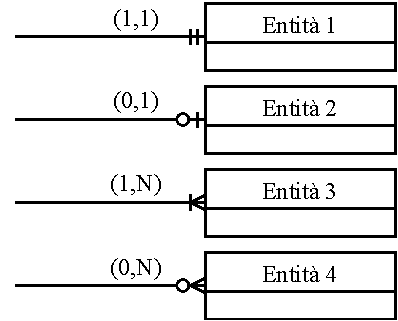
\includegraphics{assets/03/crow.pdf}
\caption{Notazione \textit{Crow's foot}.}
\label{fig:crow}
\end{wrapfigure}

\paragraph{Notazione Crow's foot} Per la realizzazione del diagramma concettuale e relazionale è stata utilizzata la notazione \textit{Crow's foot}, che rappresenta le entità come rettangoli, le quali possono avere degli attributi, e le associazioni come linee che collegano i rettangoli. La cardinalità e l'opzionalità delle associazioni si può indicare con una combinazione di specifici simboli alle estremità delle linee. I simboli utilizzati sono: l'\textbf{anello} che indica l'opzionalità, la \textbf{linea} che indica la molteplicità singola e la \textbf{zampa} che indica la molteplicità multipla. Tali simboli possono essere combinati per formare quattro tipologie di cardinalità mostrate nella figura \ref{fig:crow}. Nei diagrammi progettati vengono utilizzate tutte le cardinalità tranne la (1, N).

\paragraph{Differenza dei diagrammi} I due diagrammi, pur se sono esteticamente simili, svolgono funzioni diverse: il primo è un diagramma astratto del dominio di studio, che può essere implementato in modo diverso, per esempio in un database a oggetti o anche NoSQL, quindi non relazionale, mentre il secondo è un diagramma più vicino al database di riferimento, nel caso specifico relazionale. Il vantaggio di questa separazione è nella maggiore flessibilità nel primo diagramma, potendo esplorare e descrivere il dominio in maniera molto più libera.

\paragraph{Diagramma concettuale} La figura \ref{fig:diagramma_concettuale} mostra il diagramma concettuale, una visione ad alto livello che coinvolge soltanto entità, relazioni e attributi. In questo livello non è necessario specificare eventuali chiavi primarie, poiché verranno scelte nel passo successivo. Degli attributi elencati non viene specificata la cardinalità. Viene utilizzato il concetto di generalizzazione completa per l'entità \texttt{Message}: un'istanza di \texttt{Message} deve essere un'istanza esattamente di \texttt{Slider}, \texttt{Text} o \texttt{Image} in modo esclusivo. Rispetto alle altre entità, \texttt{Earthquake} è l'unica che è preesistente nel modello; i suoi attributi sono stati nascosti poiché non utilizzati.

\begin{figure}[ht!]
\centering
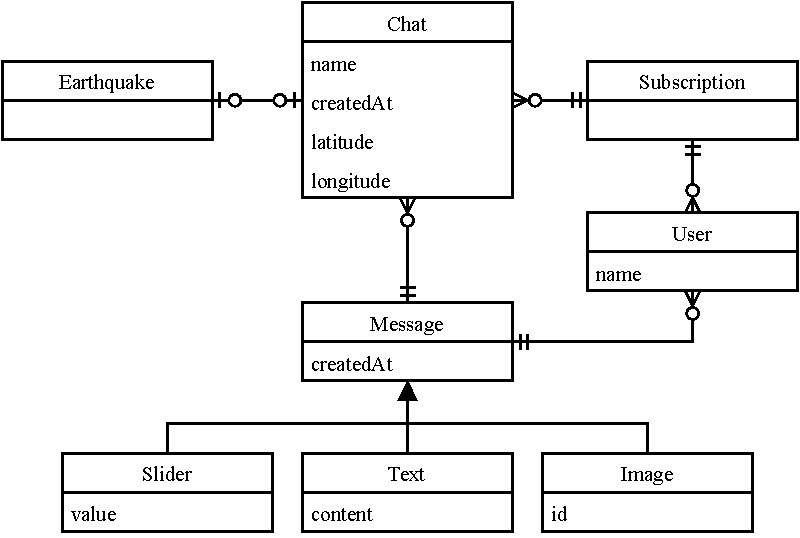
\includegraphics[width=\textwidth]{assets/03/concettuale.pdf}
\caption{Diagramma concettuale.}
\label{fig:diagramma_concettuale}
\end{figure}

\paragraph{Diagramma relazionale} Il diagramma concettuale è stato in seguito ristrutturato tenendo in mente il modello relazionale, in particolare quello implementato da MariaDB. In questo livello vengono specificate le cardinalità degli attributi, che sono del tipo (1,1) o (0,1) in base alla presenza o meno del simbolo \texttt{+}. Vengono assegnati i tipi degli attributi, senza però scendere a un livello troppo dettagliato. Sono state specificate le chiavi primarie per ogni relazione, indicando in caso di interi l'opzione di incremento automatico a ogni inserimento. Il risultato è mostrato nella figura \ref{fig:diagramma_relazionale}. Non essendo supportato il concetto di generalizzazione, si è deciso di unificare tutte le entità figlie di \texttt{Message} in una unica con l'attributo \texttt{type} che funziona da discriminante. Gli attributi \texttt{id} e \texttt{content} sono stati unificati, poiché assumono lo stesso tipo, cioè una stringa. Viene garantito, tramite l'aggiunta di un vincolo, che in base all'attributo discriminante, il corrispettivo \texttt{textcontent} o \texttt{intcontent} non sia nullo.

\paragraph{Codice SQL} Una volta ristrutturato il diagramma in modo da essere implementato in un database relazionale, la conversione in SQL è immediata. Il frammento di codice \ref{listing:diagramma_sql} mostra la conversione in SQL solo dell'entità \texttt{Chat}. Nella conversione, oltre a precisare la tipologia di dato in base alla disponibilità del database, sono state seguire le convenzioni utilizzate dalle altre tabelle in SeismoCloud, a esempio nei campi testuali e nella scelta del tipo per numeri a virgola mobile. Ogni colonna è stata rigorosamente commentata (non mostrato nel frammento), in modo da risultare il più possibile chiaro da parte di altre persone del team. Sono stati implementati direttamente in SQL i vincoli più semplici che coinvolgono la riga stessa; gli ulteriori vincoli complessi sono gestiti direttamente dall'applicativo.

\begin{listing}
\begin{minted}{sql}
CREATE TABLE `chat` (
    `id`           bigint unsigned AUTO_INCREMENT,
    `name`         varchar(255)                   NOT NULL,
    `createdat`    datetime                       NOT NULL,
    `closed`       boolean                        NOT NULL,
    `latitude`     double                         NOT NULL,
    `longitude`    double                         NOT NULL,
    `earthquakeid` int(10) unsigned,
    PRIMARY KEY (`id`),
    UNIQUE KEY (`earthquakeid`),
    CONSTRAINT `chatEarthquakeid` FOREIGN KEY (`earthquakeid`) REFERENCES `events` (`id`) ON DELETE CASCADE ON UPDATE CASCADE
) ENGINE=InnoDB DEFAULT CHARSET=utf8;
\end{minted}
\caption{Implementazione SQL del modello.}
\label{listing:diagramma_sql}
\end{listing}

\begin{figure}[ht!]
\centering
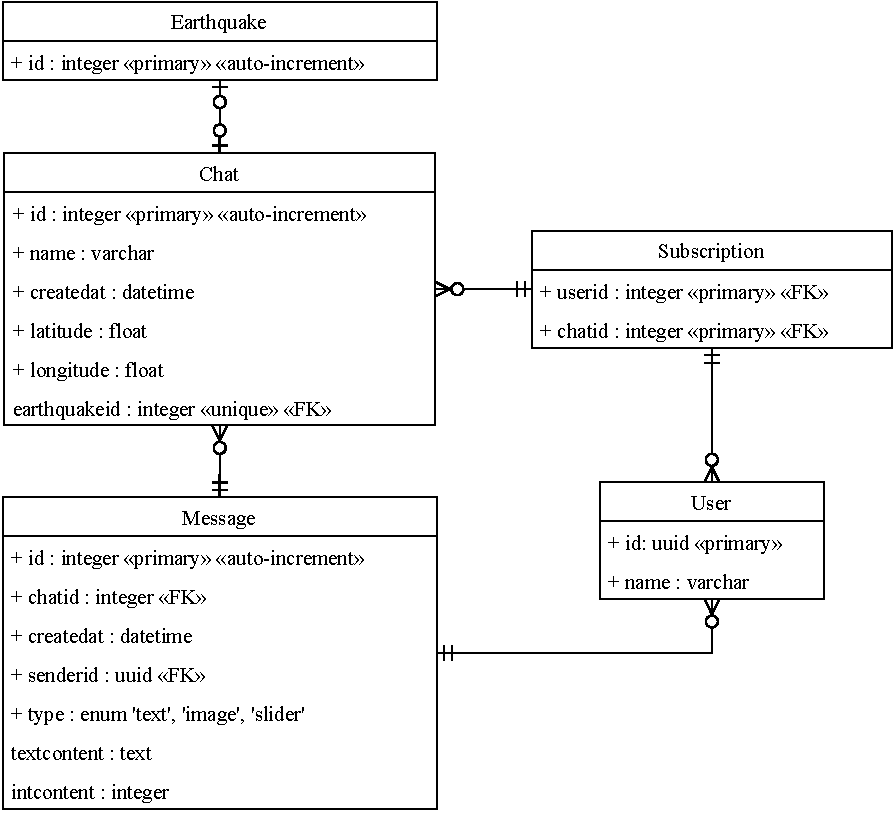
\includegraphics[width=\textwidth]{assets/03/relazionale.pdf}
\caption{Diagramma relazionale.}
\label{fig:diagramma_relazionale}
\end{figure}
